\section{The Proposed H-SFP Framework}
\label{sec:methodology}
We propose H-SFP, a three-tier framework designed to holistically address the FL trilemma: statistical heterogeneity, system heterogeneity, and communication bottlenecks. H-SFP's core innovation is a decoupled, generative workflow that severs the tight coupling of end-to-end backpropagation. Each tier (client, edge, cloud) trains independently: it ``packages'' its learned representations into lightweight feature statistics (mean and standard deviation) and transmits only these statistics upward. Additionally, the concrete algorithms for each tier are presented in Appendix A.

\begin{figure*}[t]
    \centering
    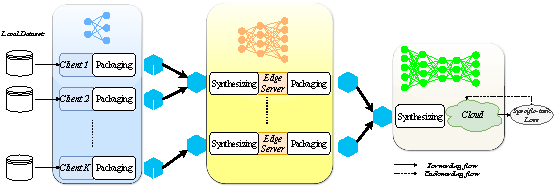
\includegraphics[width=\linewidth]{CVPR-2026/Figures/method-2.pdf}
    \caption{The H-SFP Hierarchical Architecture and Data Flow. Our framework is a three-tier system (Client, Edge, Cloud). Clients perform local training (detailed in \cref{fig:method-p1}) and ``package" their feature statistics to be sent to an Edge Server. The Edge Server uses these statistics to synthesize its own training data, trains its model segment, and then packages its own feature statistics for the Cloud. The Cloud repeats the synthesis process to train the final, task-specific model layers, eliminating the need for end-to-end backpropagation.}
    \label{fig:method-p2}
\end{figure*}

% \TODO{From my oppinion, 3.2 is a little bit verbose, 3.4 is redundant.}

\subsection{System Architecture and Model Partitioning}
\label{subsec:system_model}
% \TODO{In this part, please focus on Problem definition and system architecture. Please follow 2.1 of https://arxiv.org/pdf/2409.18448 
% Remember to note the three-tier or something else of yours, with your notation definitions.
% }

\begin{figure}[t]
    \centering
    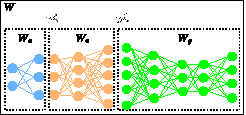
\includegraphics[width=\linewidth]{CVPR-2026/Figures/method-3.pdf}
    \caption{Model Partitioning in H-SFP. The global model $W$ is strategically split into three disjoint segments corresponding to the architectural tiers: the lightweight client-side model ($W_c$), the intermediate edge-side model ($W_e$), and the final cloud-side model ($W_g$). This partitioning offloads the primary computational burden from resource-constrained clients.}
    \label{fig:method-p3}
\end{figure}
We consider a three-tier ``cloud-edge-client'' architecture (\cref{fig:method-p2}), comprising a global cloud server, $M$ edge servers, and $K$ clients. Clients are partitioned into $M$ disjoint clusters $\{\mathcal{C}_m\}_{m=1}^M$, with each client $k \in \mathcal{C}_m$ associated with its parent edge server $m$. This hierarchical topology directly addresses the scalability and single-point-of-failure bottlenecks of centralized FL. Instead of a single cloud bottleneck processing updates from all $N$ clients, each of the $M$ edge servers performs intermediate aggregation for its local cluster. The cloud, in turn, only aggregates the $M$ processed results from the edges, significantly reducing communication overhead and latency. To address system heterogeneity (i.e., client computational constraints), H-SFP integrates split learning \cite{GUPTA20181, vepakomma2019split}. As shown in \cref{fig:method-p3}, the global model $W$ is partitioned into three disjoint segments corresponding to the tiers: lightweight client-side extractors ($W_c$), intermediate edge-side models ($W_e$), and final cloud-side layers ($W_g$). This partitioning strategy solves the computational bottleneck, as resource-constrained clients are only responsible for executing the small $W_c$ segment.

\subsection{Motivation}
    \begin{figure}[h]
        \centering
        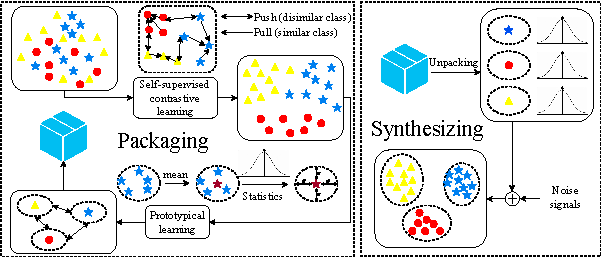
\includegraphics[width=\linewidth]{CVPR-2026/Figures/method-1.pdf}
        \caption{The Core Generative Prototyping Mechanism. This diagram illustrates the process at each tier. (Left) On clients, self-supervised contrastive learning (pulling similar, pushing dissimilar) is used to learn robust feature representations. (Right) Instead of communicating high-dimensional gradients, clients ``package" these representations into lightweight statistical moments (mean $\mu$ and std $\sigma$). These statistics (prototypes) are then used by the next tier to ``synthesize" new feature data, enabling decoupled and communication-efficient training.}
        \label{fig:method-p1}
    \end{figure}
    While SL successfully addresses the computational bottleneck, it introduces a critical communication bottleneck. In SFL, the model segments remain tightly coupled, requiring a full end-to-end backpropagation pass for every iteration. This necessitates the frequent, high-volume transmission of intermediate activations and gradients, a process that is impractical and defeats the goal of an efficient FL. To make communication efficient, two key challenges must be addressed: (i) reducing the training of the subnetworks to remove the synchronous, end-to-end backpropagation, and (ii) an alternative form of knowledge transfer that is lightweight yet semantically meaningful.
    
    Therefore, we propose a novel multi-tier generative prototyping mechanism, as illustrated in \cref{fig:method-p2} and \cref{fig:method-p1}. This feed-forward workflow completely decouples the training of the model segments ($W_c, W_e, W_g$), solving the communication and synchronization bottlenecks of SFL. To prevent long-term client drift, which can degrade purely generative approaches, our framework integrates this fast-timescale prototype exchange with a slow-timescale periodic averaging of the client-side feature extractors ($W_c$). This creates a robust hybrid system that is both communication-efficient and stable. In \cref{sec:multi_tier_learning}, we detail the independent, self-supervised learning objective for each tier. In \cref{sec:transmission_augmentation}, we describe the core mechanics of this workflow: how each tier ``packages'' its learned representations into lightweight statistics, and how the next tier ``synthesizes" a new feature dataset, $D_{syn}$, from these statistics to serve as its own training input.

\subsection{Multi-tier Self-Learning} 
\label{sec:multi_tier_learning}
    H-SFP decouples the training of the network segments, enabling each tier to learn independently. This is achieved via a multi-tier generative process where feature statistics, not gradients, are passed unidirectionally up the hierarchy.
    
    The first tier of learning occurs on the resource-constrained clients. As shown in \cref{fig:method-p1}, each client $k$ trains its local feature extractor $W_c$ using only its private data $\mathcal{D}_k$. The objective $\mathcal{L}_k(W_c)$ is to learn a high-quality, robust representation space using a self-supervised contrastive loss. Specifically, we use the NT-Xent loss \cite{chen2020simple}. For a batch $B$, let $z_i = W_c(x_i)$ be the feature embedding for a sample $x_i$:
    \begin{multline}
        \label{eq:supcon}
        \mathcal{L}_k(W_c) = \mathcal{L}_{\text{con}, k} \\
        = \sum_{i \in B} \frac{-1}{|P(i)|} \sum_{p \in P(i)} \log \frac{\exp(z_i \cdot z_p / \tau)}{\sum_{a \in A(i)} \exp(z_i \cdot z_a / \tau)},
    \end{multline}
    where $A(i) = B \setminus \{i\}$ is the set of all other samples in the batch, $P(i) \equiv \{p \in A(i) | y_p = y_i\}$ is the set of positive samples in the batch (i.e., those with the same class label as $i$), and $\tau$ is a temperature hyperparameter. This encourages the client's model to learn a feature space where samples from the same class are pulled together, while samples from different classes are pushed apart. After local training, the client distills its learned feature space into lightweight class-wise feature statistics (e.g., class-conditional mean $\mu_k$ and standard deviation $\sigma_k$). These statistics are the only information communicated upward to the edge server (in \cref{fig:method-p2}).
    
    Then, the second tier (edge server $m$) operates without access to any real data, enabling a fully decoupled architecture. First, the edge server aggregates the statistics $\{\mu_k, \sigma_k\}$ received from its client cluster $\mathcal{C}_m$ to form a stable, cluster-level feature distribution $(\mu_m, \sigma_m)$. Second, the subsequent training process is nearly identical to the client's, but it operates on synthetically generated input. The edge server unpacks these aggregated statistics and synthesizes a new feature dataset, $D_{syn}^{edge}$. This synthetic data, generated by sampling from the cluster's distribution (using $\mu_m$ as the signal and $\sigma_m$ for perturbation), serves as the input for the edge-side model, $W_e$. The edge server then trains $W_e$ by applying the same contrastive loss (defined in \cref{eq:supcon}) on its own output representations:
    \begin{equation}
        \mathcal{L}_m(W_e) = \mathcal{L}_{\text{con}, m}(W_e(D_{syn}^{edge})).
    \end{equation}
    We deliberately select this contrastive objective over a self-supervised loss to enforce objective consistency across tiers and to learn the relative relationships between feature clusters rather than overfitting the synthetic Gaussian distributions. This results in a more robust and generalized representation for the final cloud-tier classifier. This step learns an effective transformation of the client-level features into a new, more refined representation space. Like the clients, the edge server then packages the statistics of its output features and forwards them to the cloud.
    
    Finally, the final tier repeats the synthesis process, aggregating the feature statistics from all $\mathcal{M}$ edge servers to create a global distribution and generate its own synthetic dataset, $D_{syn}^{global}$. However, its objective is different. As shown in ~\cref{fig:method-p2}, the cloud server trains the final task-specific model $W_g$ (e.g., the classifier head) using a standard supervised loss, such as cross-entropy:
    \begin{equation}
        \mathcal{L}_g(W_g) = \mathcal{L}_{\text{CE}}(W_g(D_{syn}^{global})).
    \end{equation}
    This multi-tier, generative, and feed-forward process completely breaks the reliance on end-to-end backpropagation, solving the limitations of SL-based approaches.
    

\subsection{Prototype Transmission and Augmentation}
\label{sec:transmission_augmentation}
    % --- REVISED ---
    H-SFP's novelty lies in its communication, which replaces backpropagation with a feed-forward, generative process. This involves two stages: transmitting lightweight statistics and augmenting data at the receiving tier.
    % --- END REVISED ---

    \begin{algorithm}[!h]
        \caption{H-SFP: Client-Side Training}
        \label{alg:client}
        \begin{algorithmic}[1]
        \State \textbf{Input:} Client $k$, local data $D_k$, learning rate $\eta$, epochs $E$.
        \State \textbf{Receive:} Client model $W_c$.
        \State Set $W_{c,k} \leftarrow W_c$.
        \For{epoch $e = 1$ to $E$}
            \For{batch $(x, y)$ in $D_k$}
                \State $z \leftarrow W_{c,k}(x)$ \Comment{Compute feature embeddings}
                \State $\mathcal{L}_{\text{con}} \leftarrow \text{ContrastiveLoss}(z, y)$ \Comment{See \cref{eq:supcon}}
                % <<< REVISION: Removed L_align steps
                \State $W_{c,k} \leftarrow W_{c,k} - \eta \nabla \mathcal{L}_{\text{con}}$
            \EndFor
        \EndFor
        \State Compute final local statistics $\text{Stats}_k = \{(\mu_k^{(j)}, \sigma_k^{(j)}) \mid j \in \mathcal{Y}_k\}$
        \Comment{See \cref{mean_client,std_client}}
        \State \textbf{Return:} $W_{c,k}$, $\text{Stats}_k$ to Edge Server $m$.
        \end{algorithmic}
    \end{algorithm}
    
    \subsubsection{Prototype Transmission}
    % --- REVISED ---
        Our communication mechanism is a dual-timescale hybrid, which explains the distinct cost categories in \cref{tab:comm_overhead}. Most rounds (fast timescale) involve prototype exchange, where clients send only lightweight statistics ($\mu, \sigma$) instead of costly activations. This replaces the standard SFL bottleneck and corresponds to the large `Client smashed upload' cost. Infrequently (slow timescale, interval $I_c$), model averaging of the client parameters ($W_{c,k}$) occurs in the background to combat long-term drift, corresponding to the tiny 'Client model upload' cost. A similar slow-timescale process occurs at the interval $I_e$ between the edge and cloud.

    % --- END REVISED ---
        \begin{equation}
            \mu_k^{(j)} = \frac{1}{|\mathcal{D}_k^{(j)}|} \sum_{x_i \in \mathcal{D}_k^{(j)}} W_{c,k}(x_i),
            \label{mean_client}
        \end{equation}
        \begin{equation}
            \sigma_k^{(j)} = \sqrt{\frac{1}{|\mathcal{D}_k^{(j)}|} \sum_{x_i \in \mathcal{D}_k^{(j)}} (W_{c,k}(x_i) - \mu_k^{(j)})^2}.
            \label{std_client}
        \end{equation}
    % --- REVISED ---
        The transmitted package $(\mu_k^{(j)}, \sigma_k^{(j)})$ represents the complete generative statistics for class $j$. This mechanism drastically reduces communication overhead. The cost per client is $O(J_k \times d_c)$, where $J_k$ is the class count and $d_c$ is the feature dimension. This cost is independent of dataset size and model parameters $P_c$, contrasting sharply with FedAvg's $O(P_c)$ cost and standard SFL's $O(d_c)$ cost per batch.
    % --- END REVISED ---

    \subsubsection{Prototype Augmentation}
        \begin{figure}[h]
            \centering
            % Use the path to the PDF you generated
            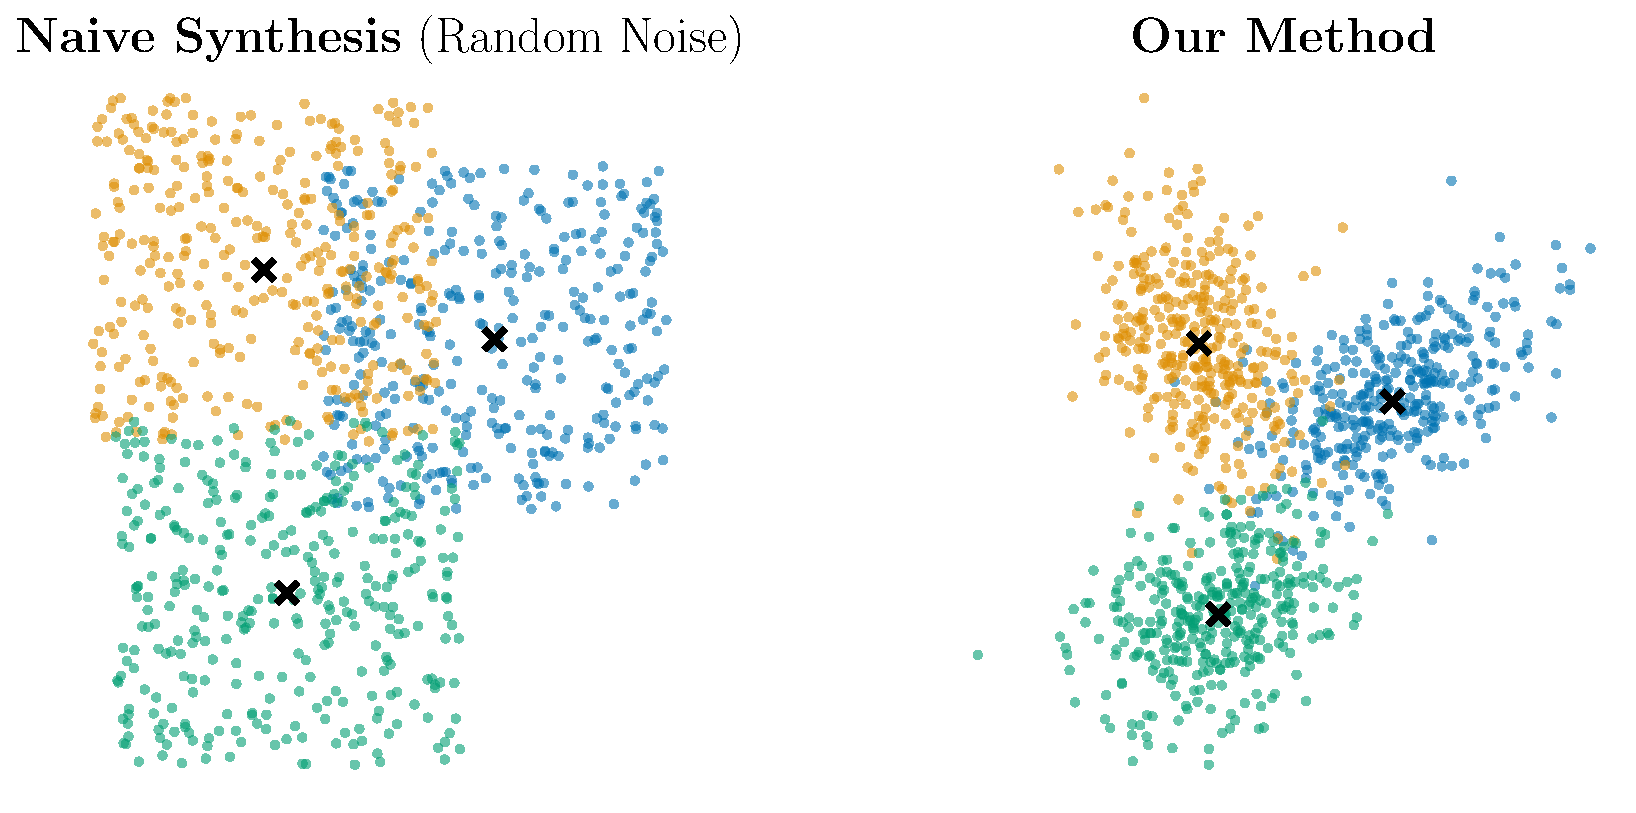
\includegraphics[width=\linewidth]{CVPR-2026/Figures/synthesis_comparison.pdf}
            \caption{Visualizing the necessity of dimension-aware generative augmentation. Real-world feature distributions are not uniform hyperballs, as variance differs across feature dimensions. This figure illustrates the impact of this fact. \textbf{(a) Naive Synthesis:} A naive approach, using only the reference vector (mean $\mu$) and simple, spherical noise, fails to capture the true, complex shape of the data distribution. \textbf{(b) Our Method:} ``Unpacking" the full transmitted statistics (both the mean $\mu$ and the standard deviation vector $\sigma$) allows for dimension-aware perturbation, which correctly reconstructs the true, elliptical shape of the feature clusters.}
            \label{fig:synthesis_comparison}
        \end{figure}
    
    % --- REVISED ---
        Upon receiving statistics $\{(\mu_k, \sigma_k)\}_{k \in \mathcal{C}_m}$, the edge server $m$ aggregates them into a cluster-level distribution:
        \begin{equation}
            \mu_m^{(j)} = \frac{1}{|\mathcal{C}_m|} \sum_{k \in \mathcal{C}_m} \mu_k^{(j)},
        \end{equation}
        \begin{equation}
            (\sigma_m^{(j)})^2 = \frac{1}{|\mathcal{C}_m|} \sum_{k \in \mathcal{C}_m} (\sigma_k^{(j)})^2.
        \end{equation}
        This distribution acts as a generative model to synthesize training data $D_{syn}^{edge}$ for the server's model segment $W_e$. As visualized in \cref{fig:synthesis_comparison}, a naive synthesis using only the mean $\mu_m^{(j)}$ and spherical noise fails, as it ignores the non-uniform, elliptical shape of true feature distributions. Our method, inspired by prototype augmentation \cite{zhu2021prototype}, recognizes this. It ``unpacks" the full statistics, using the standard deviation vector $\sigma_m^{(j)}$ to perform dimension-aware ``prototype perturbation". Specifically, a synthetic feature $z_{syn}$ for class $j$ is generated by sampling from a multivariate Gaussian by
        \begin{equation}
            \label{eq:synthesis}
            z_{syn} \sim \mathcal{N}(\mu_m^{(j)}, \text{diag}(\sigma_m^{(j)} + \epsilon)^2),
        \end{equation}
        where $\text{diag}(\cdot)$ creates a diagonal covariance matrix to model the elliptical clusters, and $\epsilon$ is a small stability constant. We intentionally use a diagonal covariance matrix as a trade-off between modeling capacity and communication cost. Our ablation study (\cref{tab:ablation}, F vs. D) confirms that modeling per-dimension variance (transmitting $\sigma$) is essential. However, transmitting a full covariance matrix would increase the communication cost from $O(d_c)$ to $O(d_c^2)$, re-introducing a major bottleneck. Our approach captures the elliptical feature distributions (\cref{fig:synthesis_comparison}) without this prohibitive cost.

    \subsection{Convergence Analysis}
        We provide convergence guarantees for H-SFP, with the full proof detailed in Appendix C. Our analysis differs from standard FL as it must account for our decoupled, generative workflow. We adopt a hierarchical, bottom-up strategy under standard non-convex assumptions (e.g., L-smoothness) and a novel $L_{stat}$-Lipschitz assumption to bound the impact of changing generative statistics. Moreover, the core of the proof is to show that the upper-tier models (edge servers and cloud) converge even while training on a ``moving target" synthetic dataset. We first prove that the client-tier statistics ($\mu_k, \sigma_k$) stabilize as the client models ($W_c$) converge. This stabilization ensures the ``distribution shock" at the edge servers diminishes ($\delta_m^t \rightarrow 0$), allowing the edge model ($W_e$) to converge. This logic extends to the cloud, confirming that the average squared gradient norm at each tier converges to a bounded neighborhood, thus proving the stability of our framework.